


\section{Projektnotizen}

Austausch und Zusammenarbeit erfolgte auf verschiedenen Platformen:
\begin{itemize}
    \item Gezeichnet und Entwürfe wurden meist in Miro\footnote{Siehe \url{https://miro.com/app/board/uXjVOdN2haQ=/}} erstellt.
    \item Besprechungen erfolgten meist in Teams\footnote{Siehe \url{https://teams.microsoft.com/l/team/19\%3aDoBvOwOIC6WNhsL9kOIYFKNtVftU1yBtcEn_gcyQtcg1\%40thread.tacv2/conversations?groupId=850a22ff-34a2-4fe2-a506-f55ac4d595f8&tenantId=b9b6f99a-a243-422d-ab36-f726574c981a}}. 
    \item Der gemeinsame Code und die Dokumentation wurden auf Github erstelt: \url{https://github.com/tstsrv-de/rpg}. 
\end{itemize}




\section{Ideen für Erweiterungen über diese Projektarbeit hinaus (Ausblick)} \label{ausblick}

Da der Umfang dieser Projekt beschränkt ist, können nicht alle erdachten Funktionen umgesetzt werden. Einige Ideen, sollen aber nicht ungenannt bleiben: 
\begin{enumerate}
    \item Würfel bei Schaden bzw. Angriff implementieren.
    \item Aggrotabelle und verbundene Funktionen implementieren.
    \item Inaktive und getrennte Spieler bzw. Nutzer aus den Chatfunktionen der Weltkarte und Lobby entfernen. Ggfls. auch einen Timer für das Spiel anlegen der anderen Spielern anzeigt, wenn ein Spieler inaktiv bzw. getrennt vom Server ist. 
    \item E-Mail Funktion von Django konfigurien, damit das Zurücksetzen von Passwörtern u.A. möglich wird.
    \item Der Traefik-Proxy sollte noch um die Monitoring- und Logging-Funktionen erweitert werden. 
\end{enumerate}



\section{Notizen Erstellung Django-Anwendung} \label{django-init}

Die Django-Anwendung für dieses Projekt wurde anhand der Anleitungen und Versuche aus den Vorlesungen neu erstellt. Dabei wurden die Schritte kurz und in Stichworten notiert. Relevant dazu sind die Commits von Samstag 13.11.2021, siehe \url{https://git.io/JSq7n} und \url{https://git.io/JSYH4}. Dies als Anhang hier: 

\begin{lstlisting}1. copy files (docker-compose, dockerfile, example.env, requirements.txt) from repo local
2. rename .env.example to .env and change settings 
3. init django with: docker-compose run rpg django-admin startproject rpg .
4. edit rpg/settings.py:
    add:
        start:
            import os
            import environ
            env = environ.Env()
            environ.Env.read_env()
        after 'BASE_DIR':
            TEMPLATES_DIR = os.path.join(BASE_DIR, 'templates')
            STATIC_DIR = os.path.join(BASE_DIR, 'static')
        after STATIC_URL:
            STATICFILES_DIRS = [
                STATIC_DIR,
            ]
    change: 
        SECRET_KEY to:
            SECRET_KEY = env('ENV_SECRET_KEY')
        ALLOWED_HOSTS to:
            ALLOWED_HOSTS = [env('ENV_ALLOWED_HOSTS')]
        in Templates, Dirs to:
                'DIRS': [TEMPLATES_DIR],
        DATABASES to:
            DATABASES = {
                'default': {
                    'ENGINE': 'django.db.backends.postgresql',
                    'NAME': env('ENV_POSTGRES_DB'),
                    'USER': env('ENV_POSTGRES_USER'),
                    'PASSWORD': env('ENV_POSTGRES_PASSWORD'),
                }
            }

5. copy and rename .env.example also to rpg/.env (remeber to copy again @changes)
6. update django to new db: 'docker-compose run python manage.py makemigrations' and 'docker-compose run python manage.py migrate'
7. create superuser: docker-compose run rpg python manage.py createsuperuser
8. create django app: docker-compose run rpg python manage.py startapp rjh_rpg \end{lstlisting}
    


\section{Inhalte aus und zu Projektbesprechungen}

Stets Sonntags erfolgten Projektbesprechungen. Notizen und Zusammenfassungen davon finden sich hier in fortschreitender, chronologischer Reihenfolge (insofern diese im Hauptteil der Dokumentation nicht bereits dargetellt wurden). Ebenso hier entsprechend einsortiert, finden sich Konzeptzeichnungen und Entwürfe aller Art (UI, Code, Datenbankmodelle).


(TODO!) Bildbeschreibungen ergänzen, wichtige Bilder beschreiben.


\begin{figure}[H]
    \centering
    \caption{2021-11-23-erster-entwurf-gameloop}
    \label{fig:2021-11-23-erster-entwurf-gameloop}
    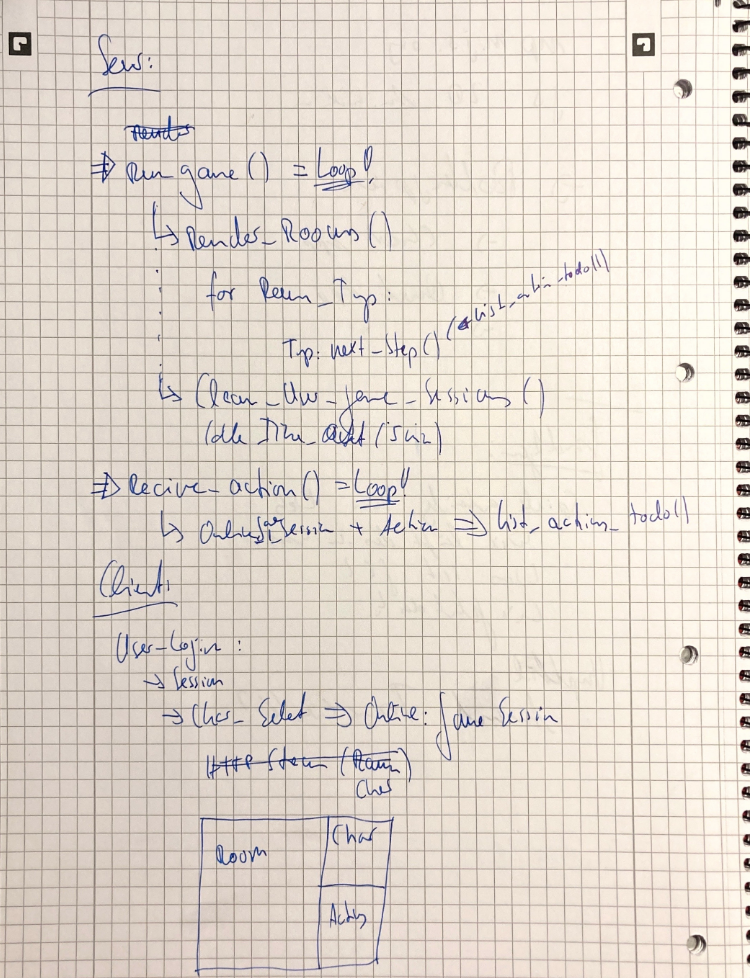
\includegraphics[width=1\textwidth]{2021-11-23-erster-entwurf-gameloop}
\end{figure}





\begin{figure}[H]
    \centering
    \caption{2021-11-27-erstentwurf-ui}
    \label{fig:2021-11-27-erstentwurf-ui}
    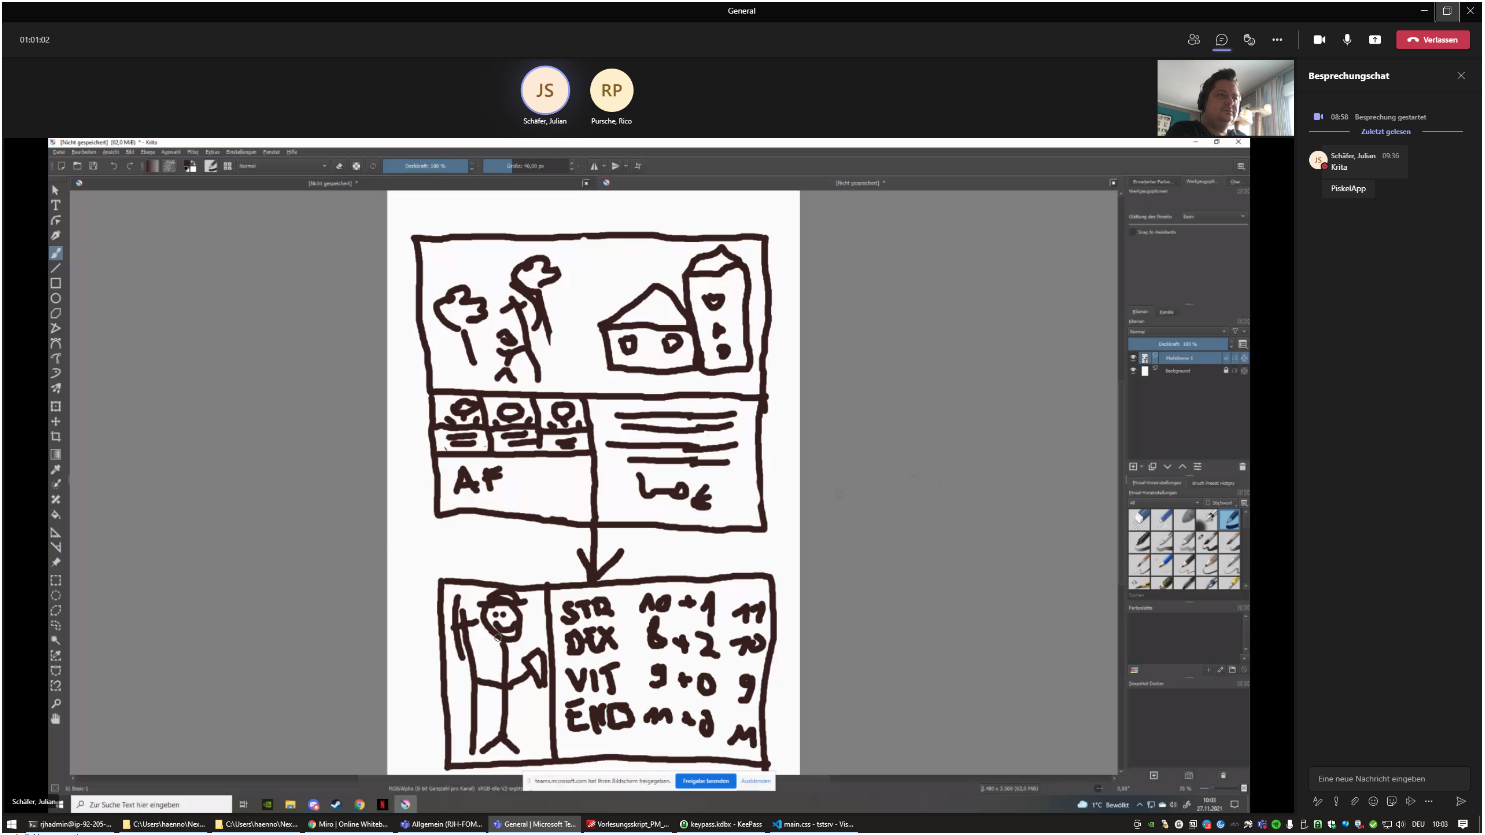
\includegraphics[width=1\textwidth]{2021-11-27-erstentwurf-ui}
\end{figure}


\begin{figure}[H]
    \centering
    \caption{2021-11-29-Entwurf-Klassen-Ui}
    \label{fig:2021-11-29-Entwurf-Klassen-Ui}
    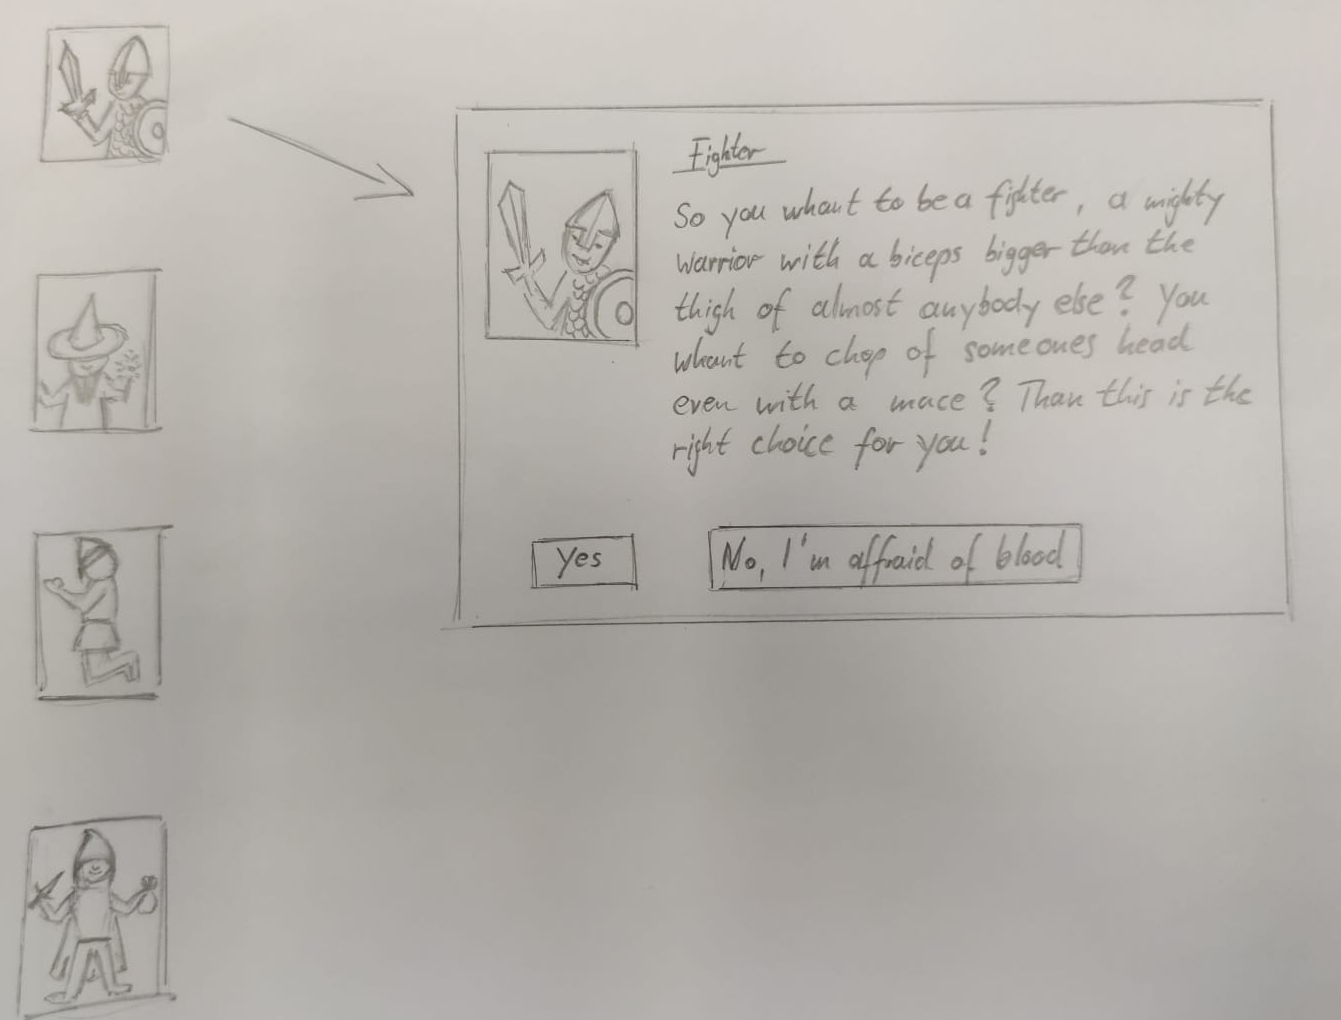
\includegraphics[width=1\textwidth]{2021-11-29-Entwurf-Klassen-Ui}
\end{figure}


\begin{figure}[H]
    \centering
    \caption{2021-11-30-Entwurf-Lobby-Logik}
    \label{fig:2021-11-30-Entwurf-Lobby-Logik}
    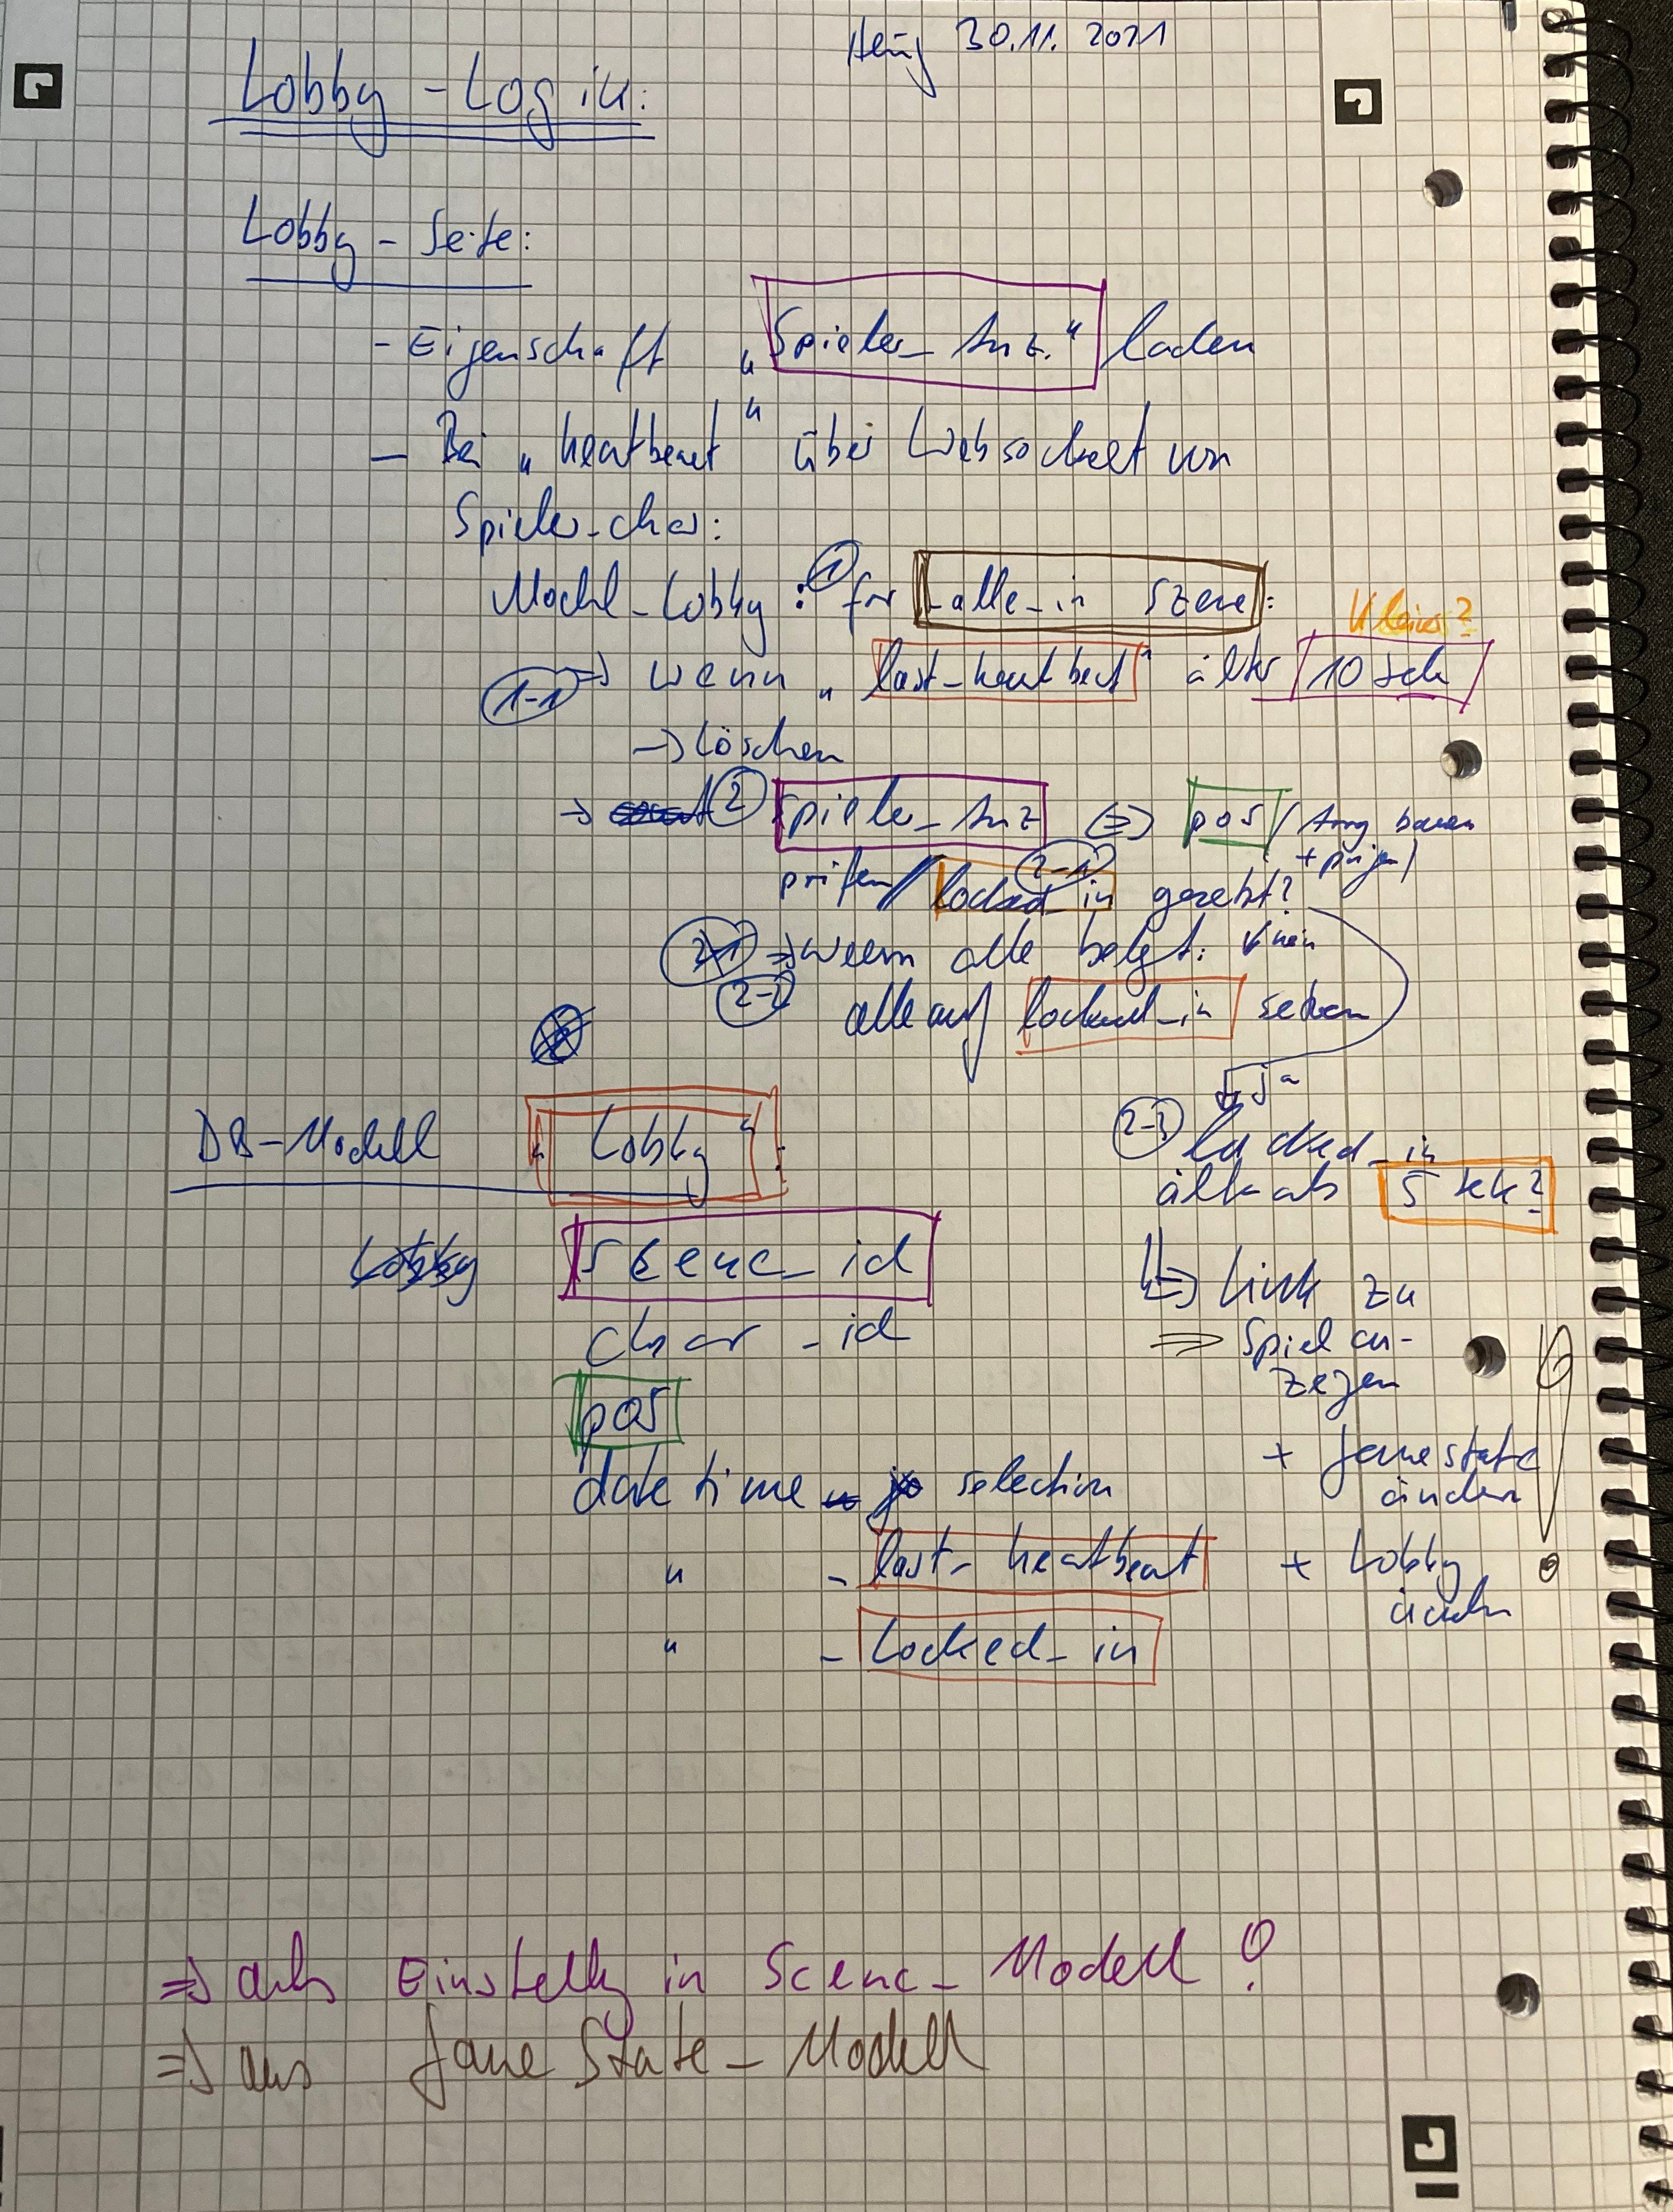
\includegraphics[width=1\textwidth]{2021-11-30-Entwurf-Lobby-Logik}
\end{figure}


\begin{figure}[H]
    \centering
    \caption{2021-11-30-Entwurf-Lobby-UI}
    \label{fig:2021-11-30-Entwurf-Lobby-UI}
    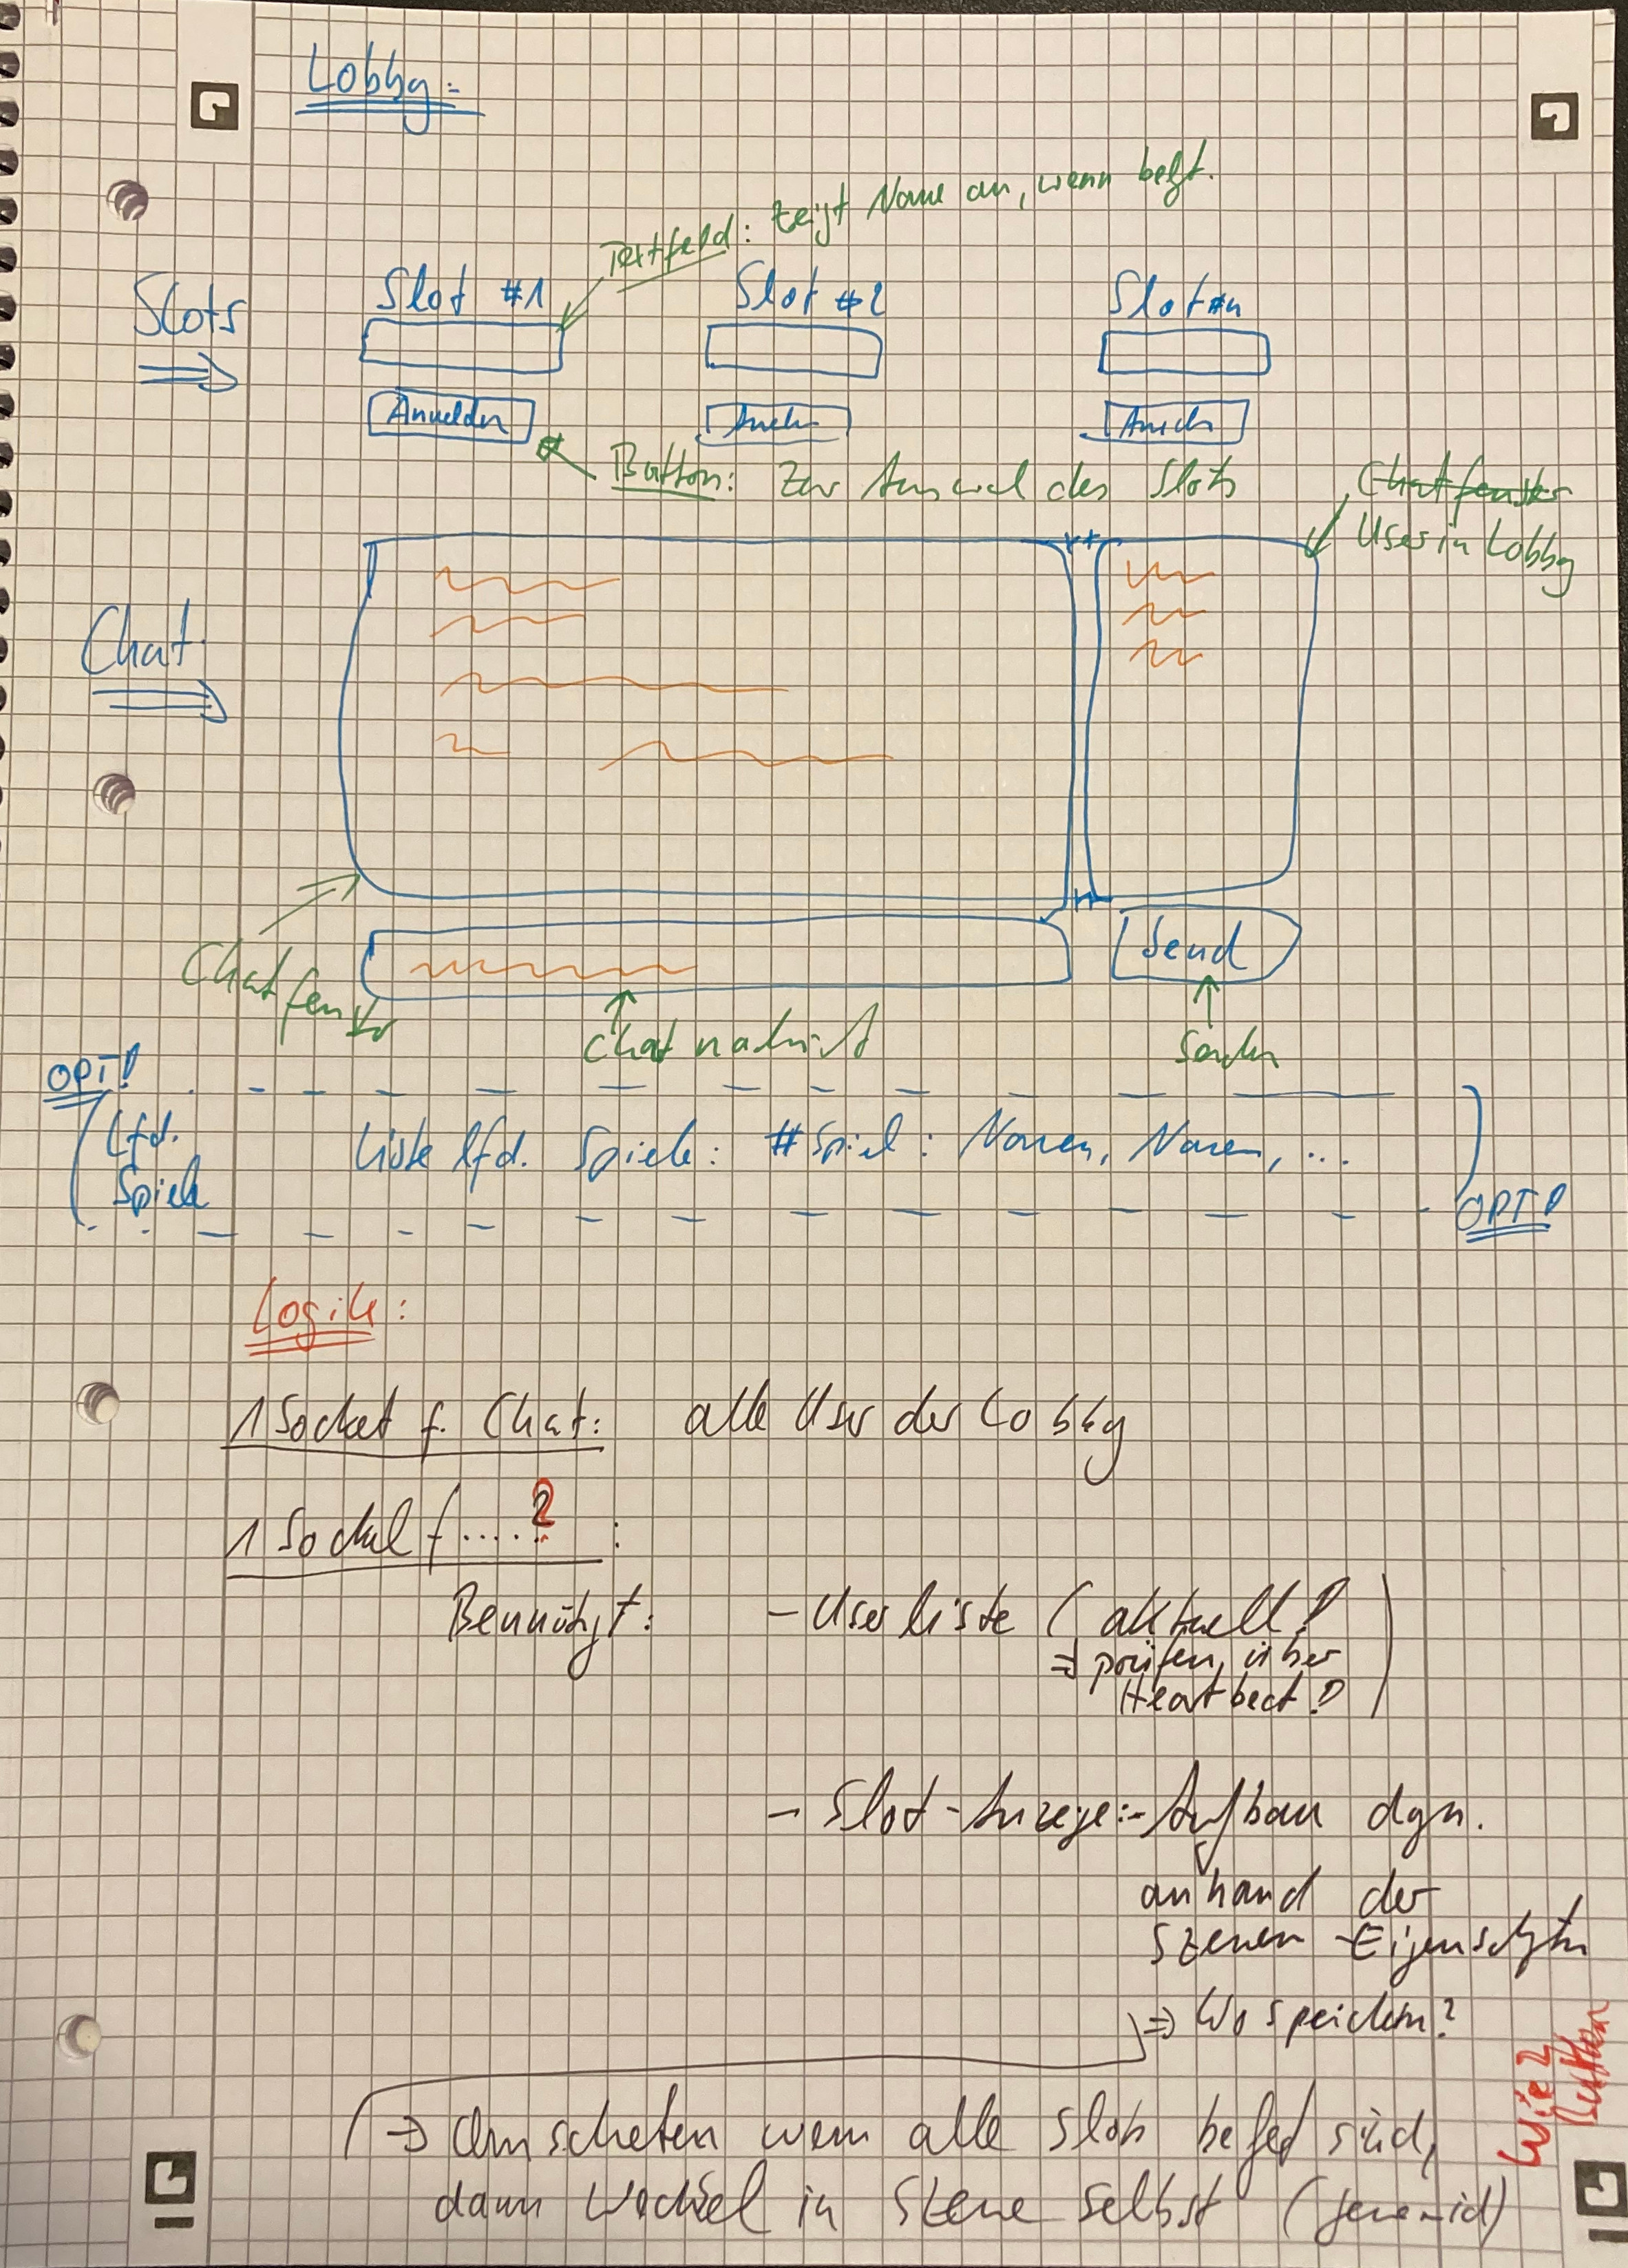
\includegraphics[width=1\textwidth]{2021-11-30-Entwurf-Lobby-UI}
\end{figure}


\begin{figure}[H]
    \centering
    \caption{2021-12-02-Countdown-Logik}
    \label{fig:2021-12-02-Countdown-Logik}
    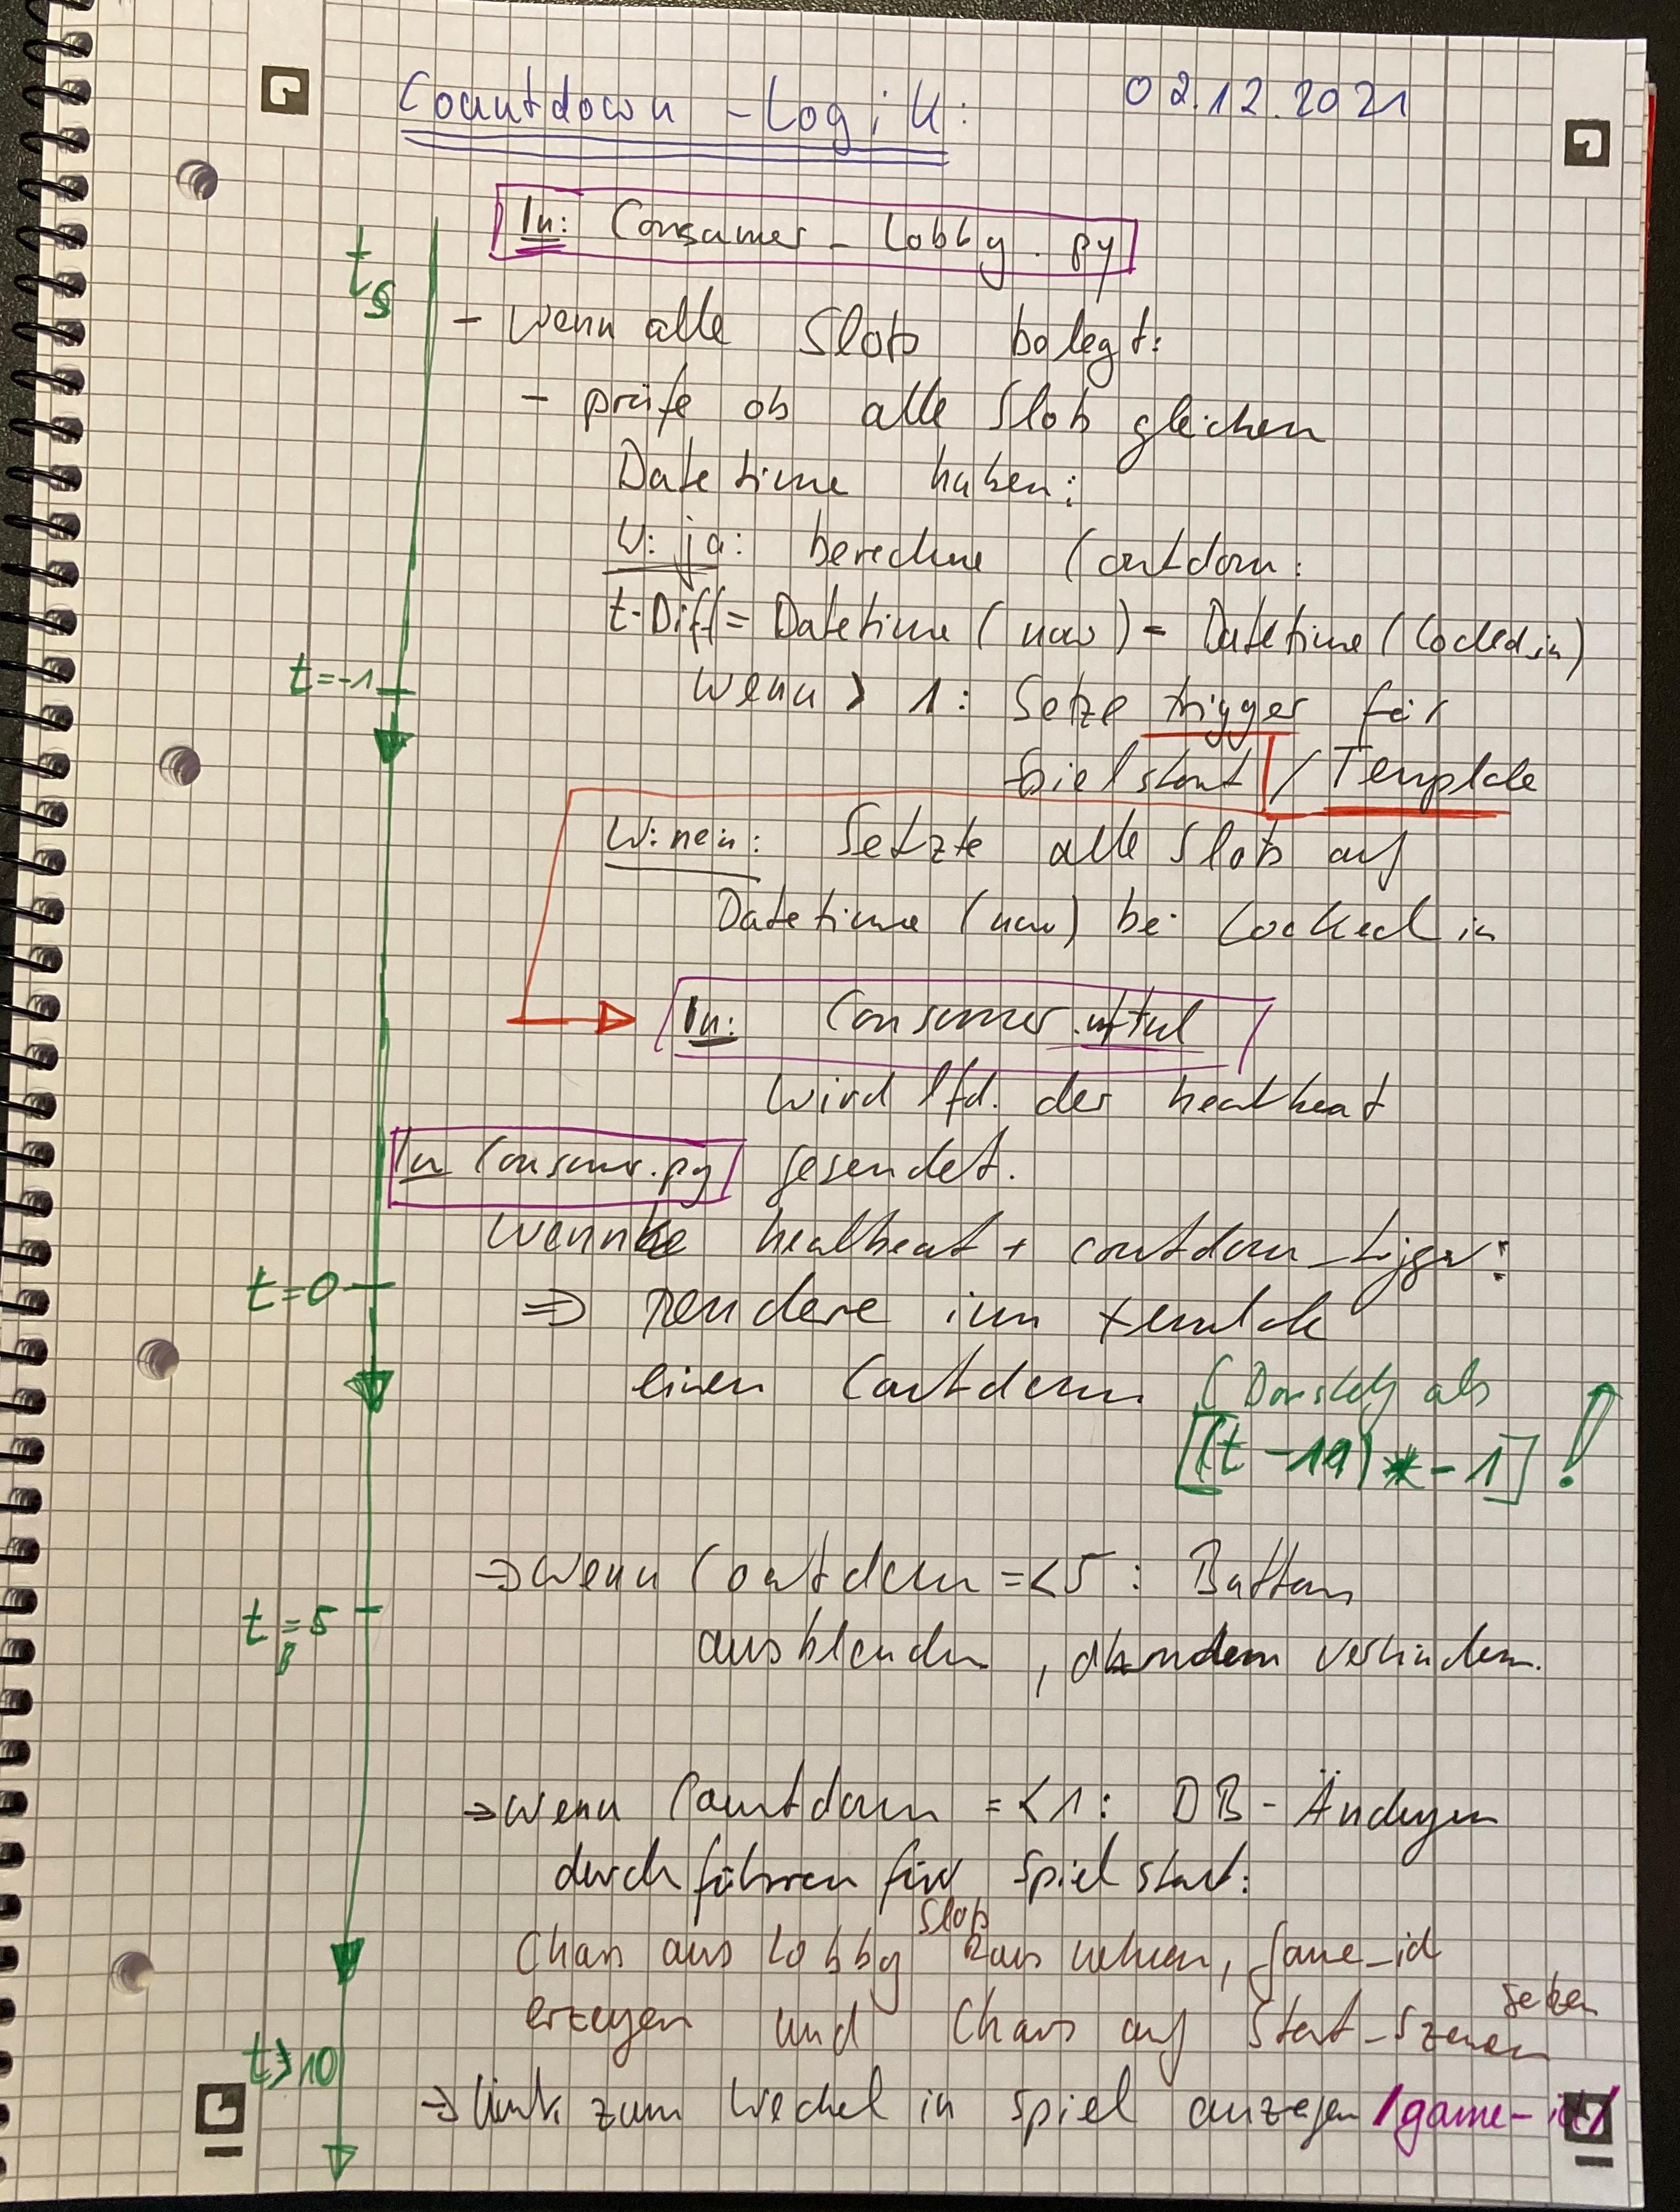
\includegraphics[width=1\textwidth]{2021-12-02-Countdown-Logik}
\end{figure}

 
\begin{figure}[H]
    \centering
    \caption{2021-12-05-Projketbesprechung-Miro-b}
    \label{fig:2021-12-05-Projketbesprechung-Miro-b}
    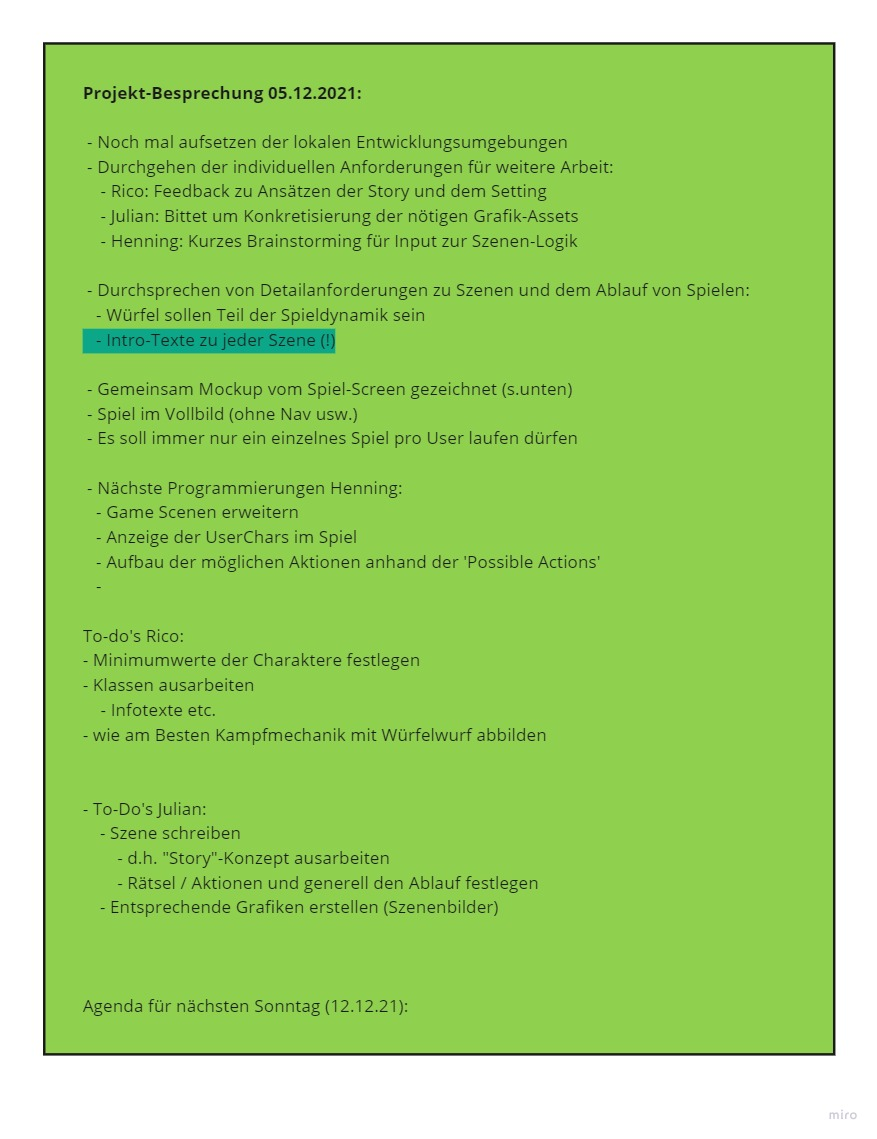
\includegraphics[width=1\textwidth]{2021-12-05-Projketbesprechung-Miro-b}
\end{figure}





\begin{figure}[H]
    \centering
    \caption{2021-12-11-Projekt-Besprechung-Klassenbeschreibung}
    \label{fig:2021-12-11-Projekt-Besprechung-Klassenbeschreibung}
    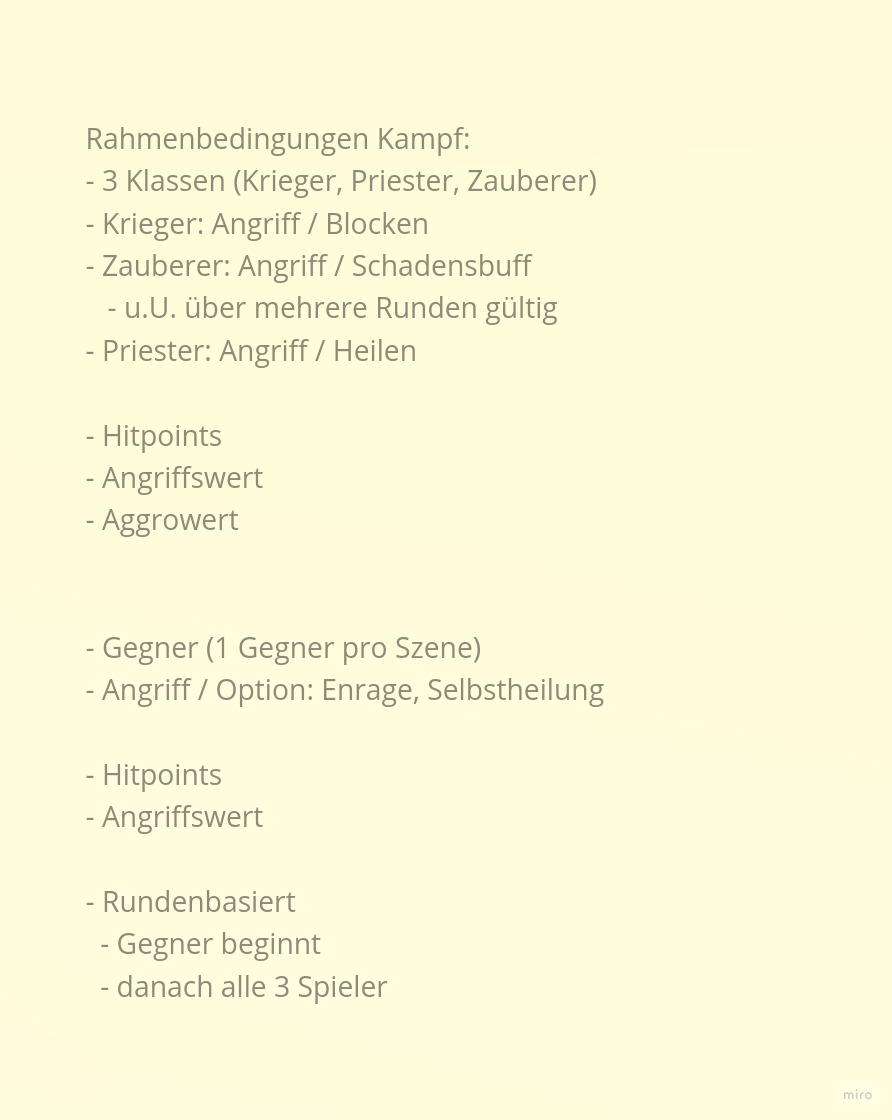
\includegraphics[width=1\textwidth]{2021-12-11-Projekt-Besprechung-Klassenbeschreibung}
\end{figure}


\begin{figure}[H]
    \centering
    \caption{11.12.2021: Projekt Besprechung: Gegenseitiges Update und Wechsel von Szenenlogik zu Kampfsystem für das RPG }
    \label{fig:2021-12-11-Projekt-Besprechung}
    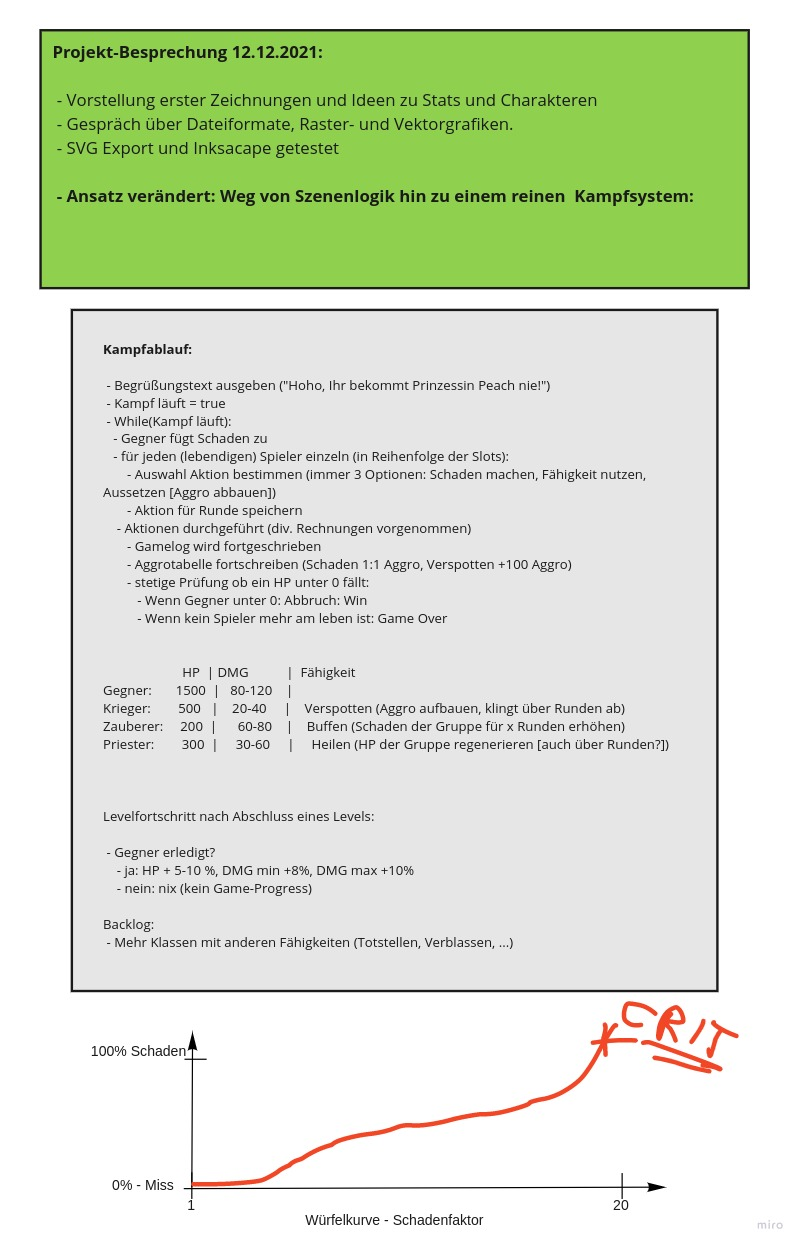
\includegraphics[width=1\textwidth]{2021-12-11-Projekt-Besprechung}
\end{figure}


\begin{figure}[H]
    \centering
    \caption{06.01.2022: Projekt Besprechung: Ermitteln von restlichen ToDos, Aufgabenverteilung, Meilienstein- und Terminplanung}
    \label{fig:2022-01-06-Projektbesprechung}
    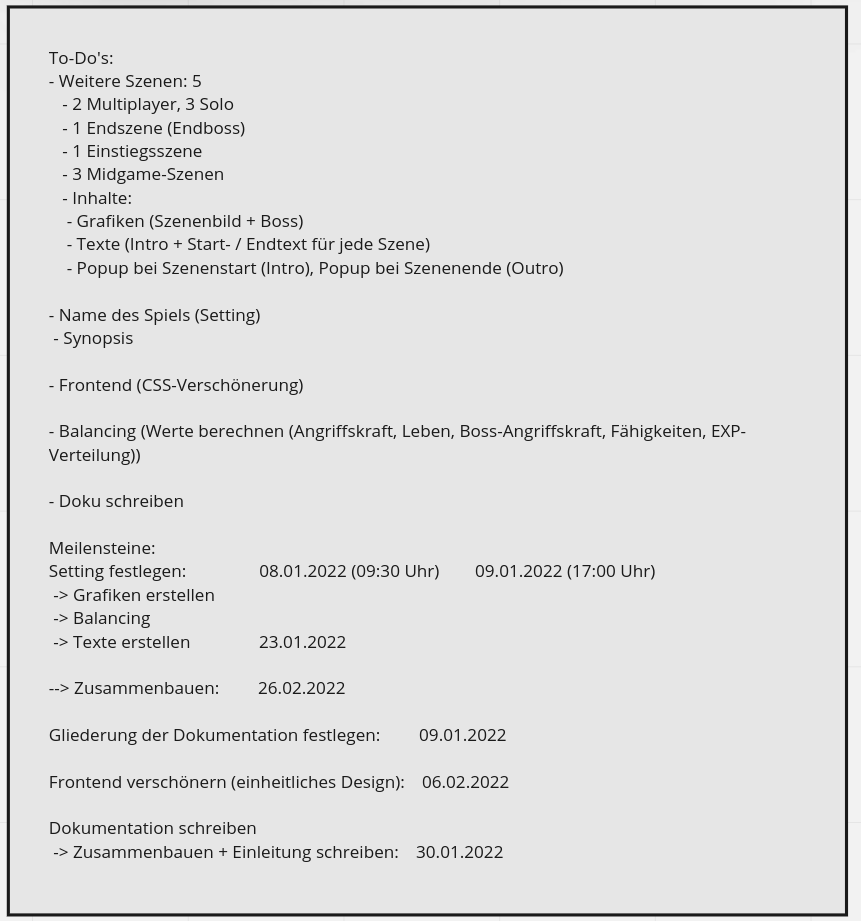
\includegraphics[width=1\textwidth]{2022-01-06-Projektbesprechung}
\end{figure}

